% --
% spectrogram

\section{Spectral Features}\label{sec:signal_spec}
Spectral Features, such as a spectrogram, are the most intuitive form to represent audio waveforms. 
They illustrate which frequencies are active at each time instance using a fixed analytic window $t_N$, shifted on the time axis with a time interval, denoted as hop time $t_{h}$.
The analytic window containing a number of $N$ audio samples, is transformed with the Discrete Time Fourier Transform (DTFT):

% DTFT
\begin{equation}\label{eq:signal_spec_dtft}
    X[k] = \sum_{n=0}^{N-1} x[n] \, e^{-j\frac{2 \pi n}{N}k}
\end{equation}
into the frequency space $X \in \C^k$ with frequency index $k$, sample index $n$ and discrete audio samples $x[n]$.
\req{signal_spec_dtft} can be conveniently written in matrix notation with:
\begin{equation}\label{eq:signal_spec_dtft_matrix}
    X[k] = D\, x[n] \quad \mathrm{with} 
    \quad D[p, q] = e^{-j\frac{2 \pi p}{N} q},
    \quad p, q = 0 \dots N-1.
\end{equation}

The length of the analytic window in samples $N$ is crucial for the frequency resolution and the lowest frequency that can be represented.
For example, the periodic time of a sound with $f=\SI{20}{\hertz}$ is $t=\frac{1}{f} = \SI{50}{\milli\second}$.
To represent a waveform it is necessary to have at least a quarter of its wavelength captured.
Within this thesis, the length of the analytic window is selected to \SI{25}{\milli\second}.

The other important parameter is the \emph{hop size} (in samples) or hop time, by which the analytical window is shifted on the time axis.
This parameter indicates the resolution in time and is especially important for changes.
In applications like speech processing, the hop time should be selected so that the fastest pronounced phone is within this time span and that changes to other phones are as well captured with sufficient resolution.
Usually a hop time of $t_{h}=\SI{10}{\milli\second}$ is chosen (also used within this thesis), but it could be extended like in \cite{Peter2020} to $t_{h}=\SI{20}{\milli\second}$ for saving computations.

With those parameters in mind and $h$ denoted as hop size in samples and $N$ the length of the analytical window, the Short-Time Fourier Transform (STFT) for discrete time signals, can be computed as:

% stft
\begin{equation}\label{eq:signal_spec_stft}
    X[m, k] = \sum_{n=0}^{N-1} x[n + m] \, w[n] \, e^{-j\frac{2 \pi n}{N}k}, \qquad m = 0 \cdot h, \, 1 \cdot h, \, \dots, \, M \cdot h 
\end{equation}
note that $n$ is here the summation index, $w$ is a window function, such as the \emph{Hanning} window, $m$ indicates the hop index and $M$ is the maximum number of hops.
The maximum number of hops $M$ are all shifts of the analytic window by the hop size on the discrete time axis and can be computed as:

% hop
\begin{equation}\label{eq:signal_spec_hop}
  M = \frac{n-N}{h}
\end{equation}
where $n$ is here the length of the discrete time signal $x$.
A summary of the STFT parameters are shown in \rtab{signal_spec_stft}.

% stft params
% --
% stft params
\begin{table}[ht!]
\begin{center}
\caption{Parameters used for the STFT computation.}
\begin{tabular}{ M{4cm}  M{4cm}}
\toprule
\textbf{Parameter} & \textbf{Value} \\
\midrule
Sampling Frequency & \SI{16}{\kilo\hertz}\\
Analytic window size & \SI{25}{\milli\second}\\
Hop size & \SI{10}{\milli\second}\\
Window Function & Hanning\\
\bottomrule
\label{tab:signal_spec_stft}
\end{tabular}
\end{center}
\end{table}
\FloatBarrier
\noindent

A spectrogram $P \in \R^{m \times k}$ is simply the power spectrum of the STFT signal and is computed with:

% spec
\begin{equation}\label{eq:signal_spec_spec}
  P[m, k] = \abs{X[m, k]}^2.
\end{equation}
A spectrogram with linear representation is shown in \rfig{signal_spec_lin_examples}.

\begin{figure}[!ht]
  \centering
    \subfigure[left]{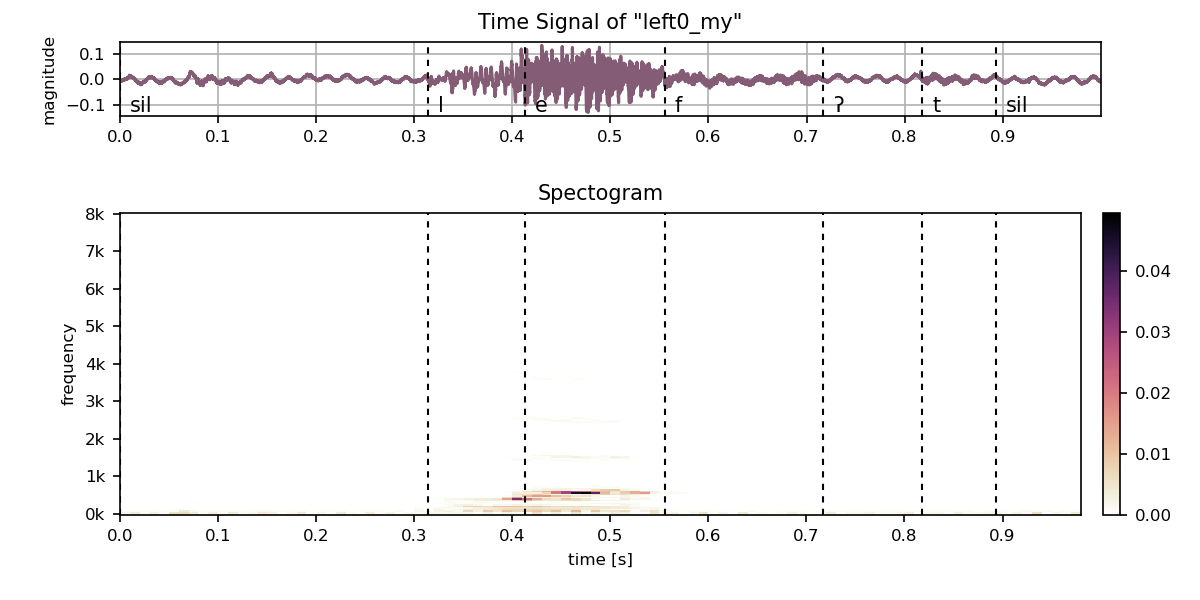
\includegraphics[width=0.45\textwidth]{./3_signal/figs/signal_spec-lin_left0_my}}
    \subfigure[right]{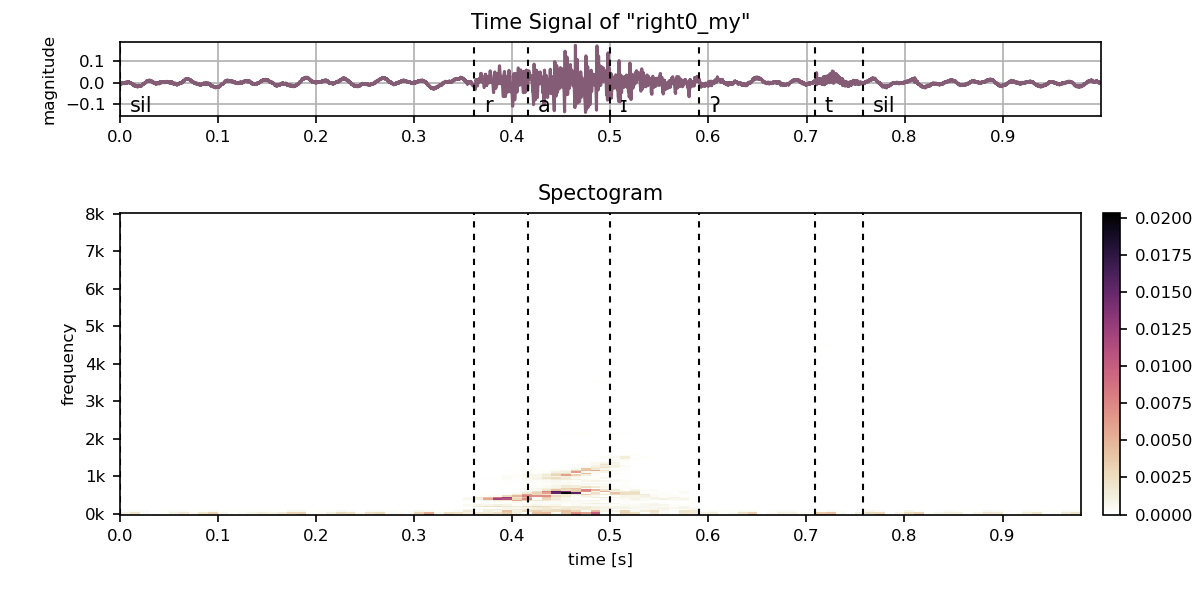
\includegraphics[width=0.45\textwidth]{./3_signal/figs/signal_spec-lin_right0_my}}
    \subfigure[up]{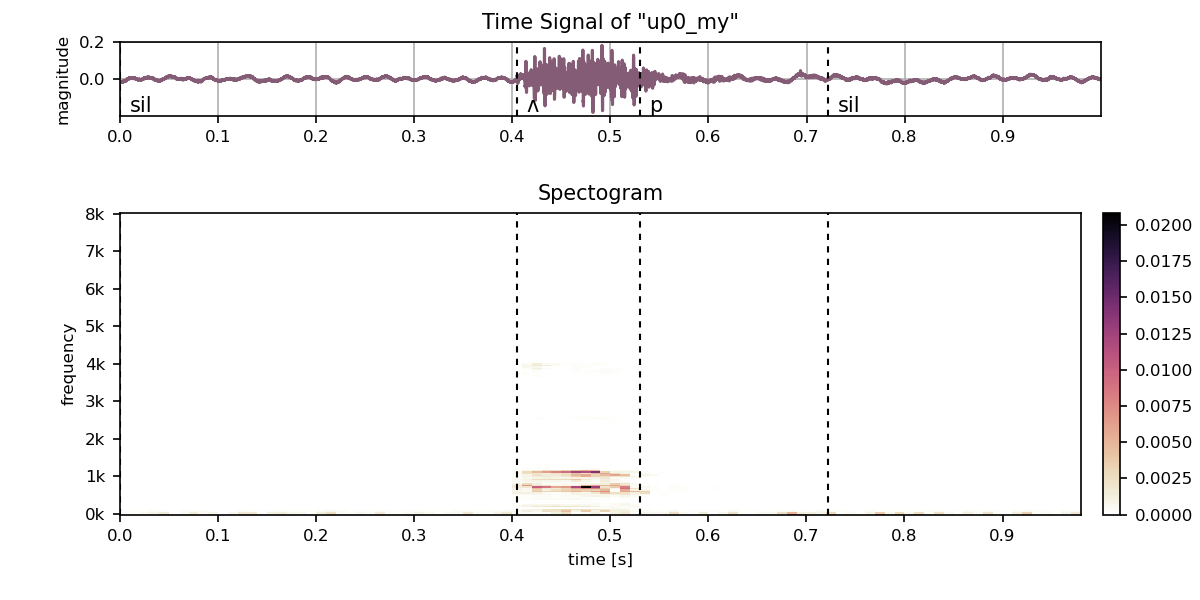
\includegraphics[width=0.45\textwidth]{./3_signal/figs/signal_spec-lin_up0_my}}
    \subfigure[down]{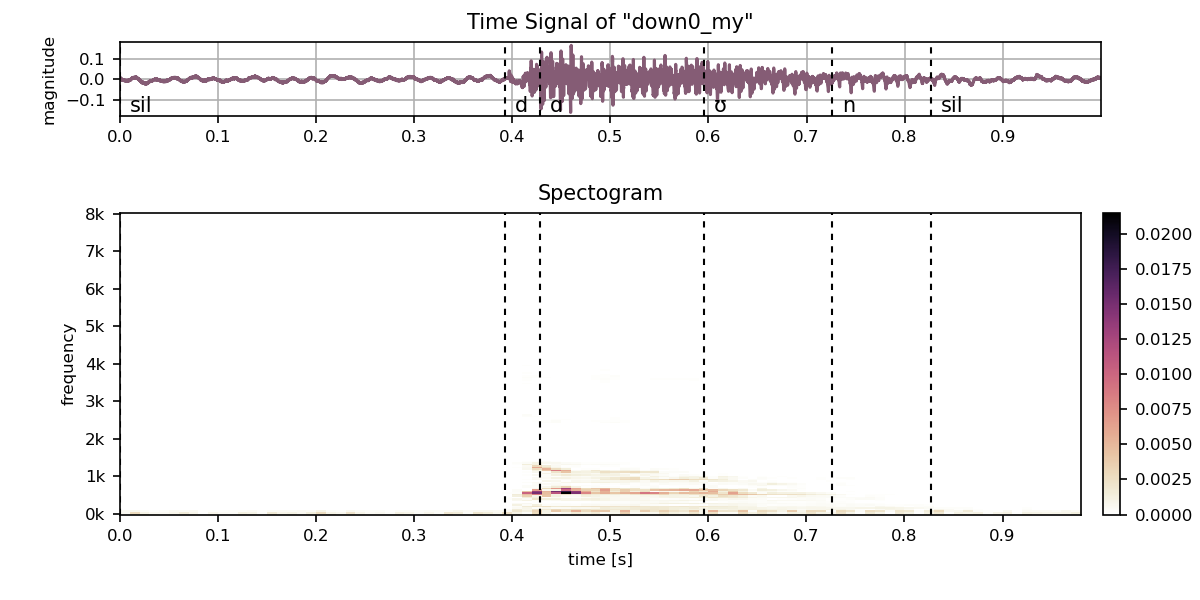
\includegraphics[width=0.45\textwidth]{./3_signal/figs/signal_spec-lin_down0_my}}
    \subfigure[go]{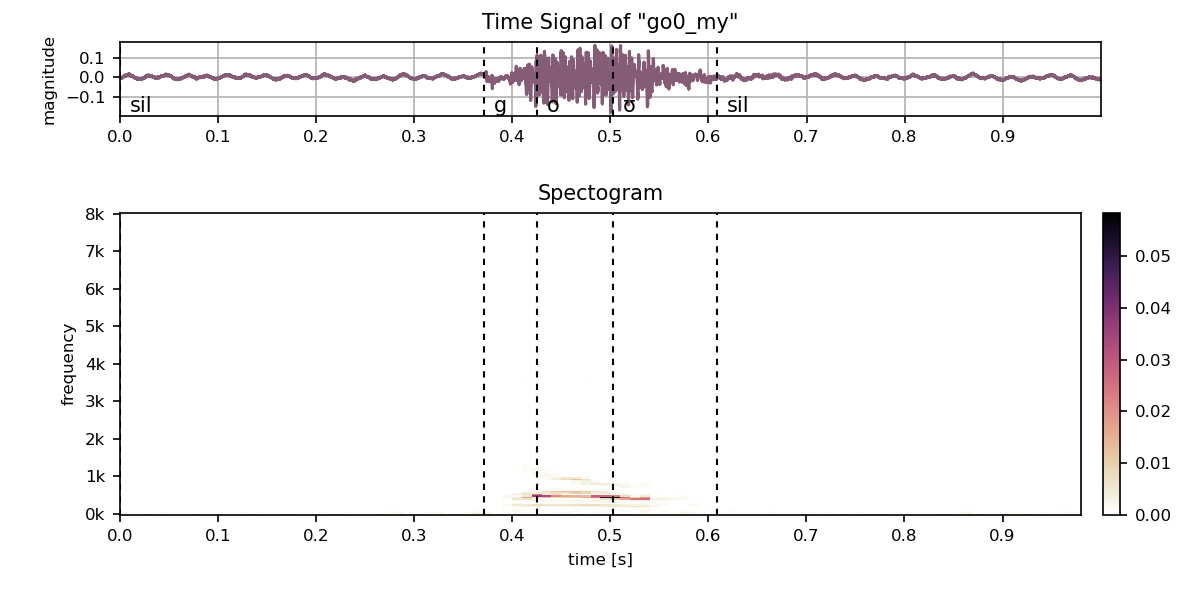
\includegraphics[width=0.45\textwidth]{./3_signal/figs/signal_spec-lin_go0_my}}
  \caption{Spectrogram linear scaled.}
  \label{fig:signal_spec_lin_examples}
\end{figure}
\FloatBarrier
\noindent

One can see here, that most of the energy of the signal is in the lower frequency regions under \SI{1}{\kilo\hertz}.
It is more interesting to transform the signal into the log scale with:

% log
\begin{equation}\label{eq:signal_spec_log}
  P_{DB}[m, k] = 10 \cdot \log{P[m, k]}
\end{equation}
so that small energies are visualized much better. 
The same examples with log scale are shown in \rfig{signal_spec_log_examples}.

\begin{figure}[!ht]
  \centering
    \subfigure[left]{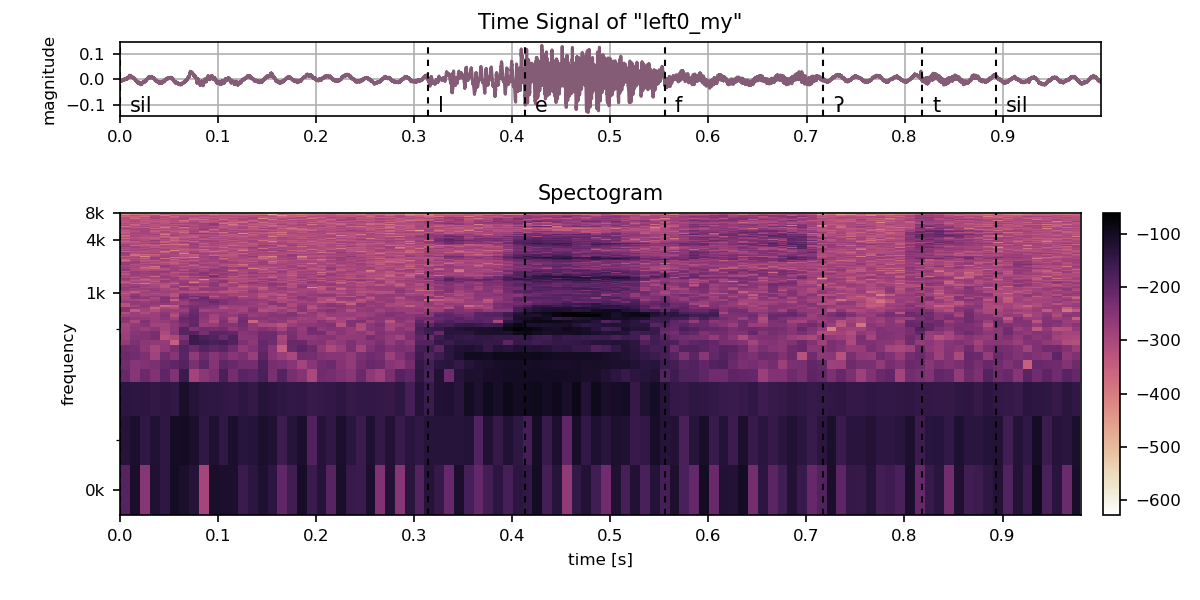
\includegraphics[width=0.45\textwidth]{./3_signal/figs/signal_spec-log_left0_my}}
    \subfigure[right]{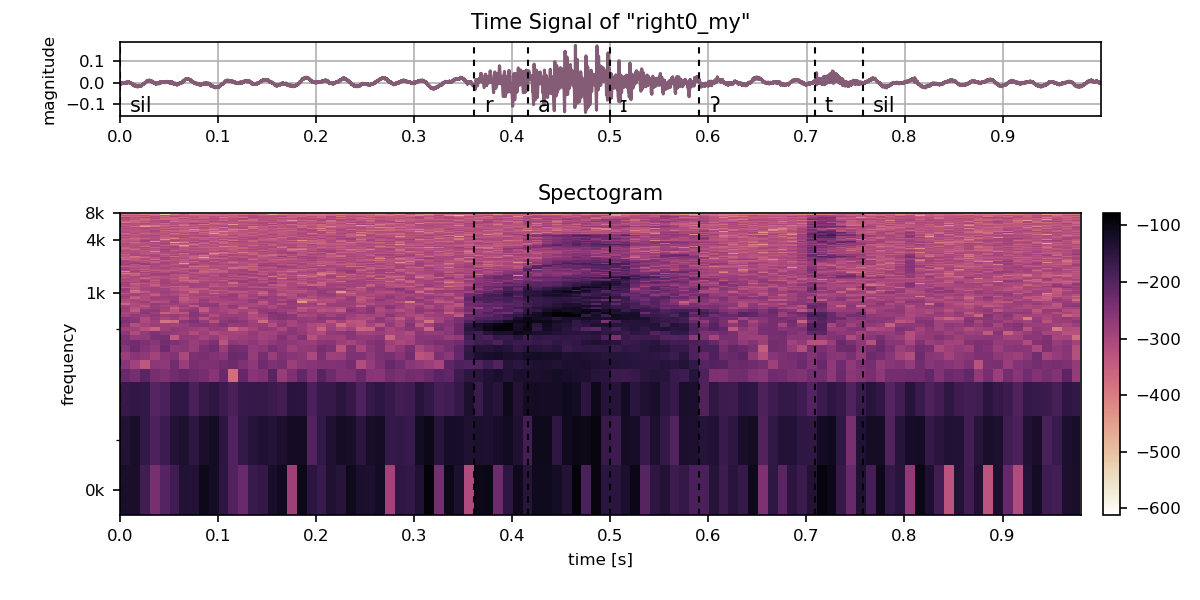
\includegraphics[width=0.45\textwidth]{./3_signal/figs/signal_spec-log_right0_my}}
    \subfigure[up]{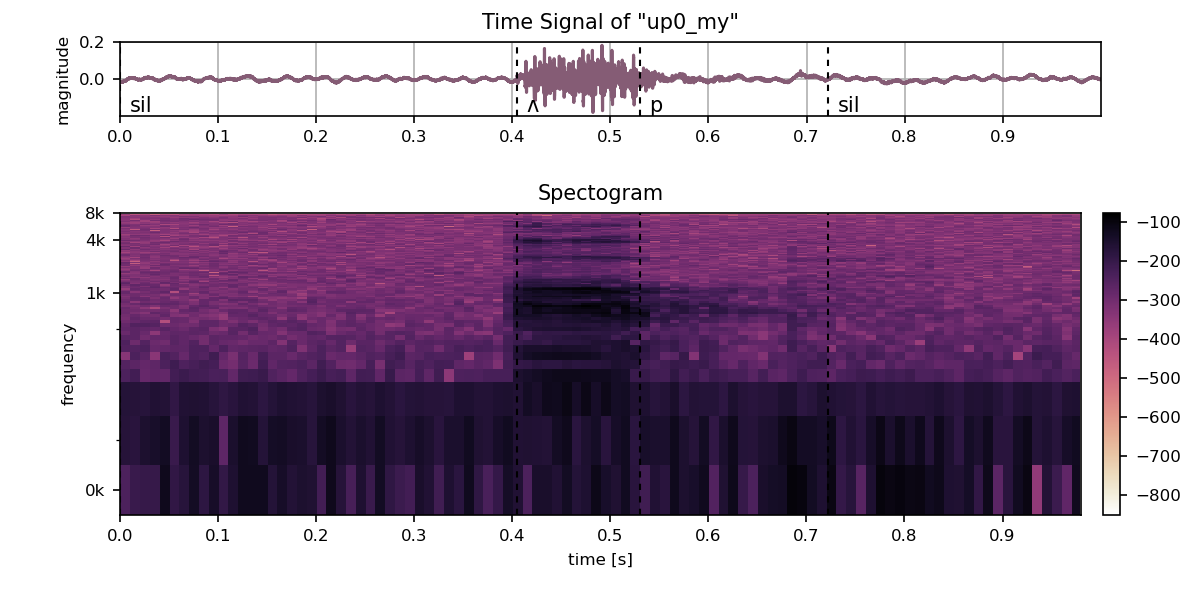
\includegraphics[width=0.45\textwidth]{./3_signal/figs/signal_spec-log_up0_my}}
    \subfigure[down]{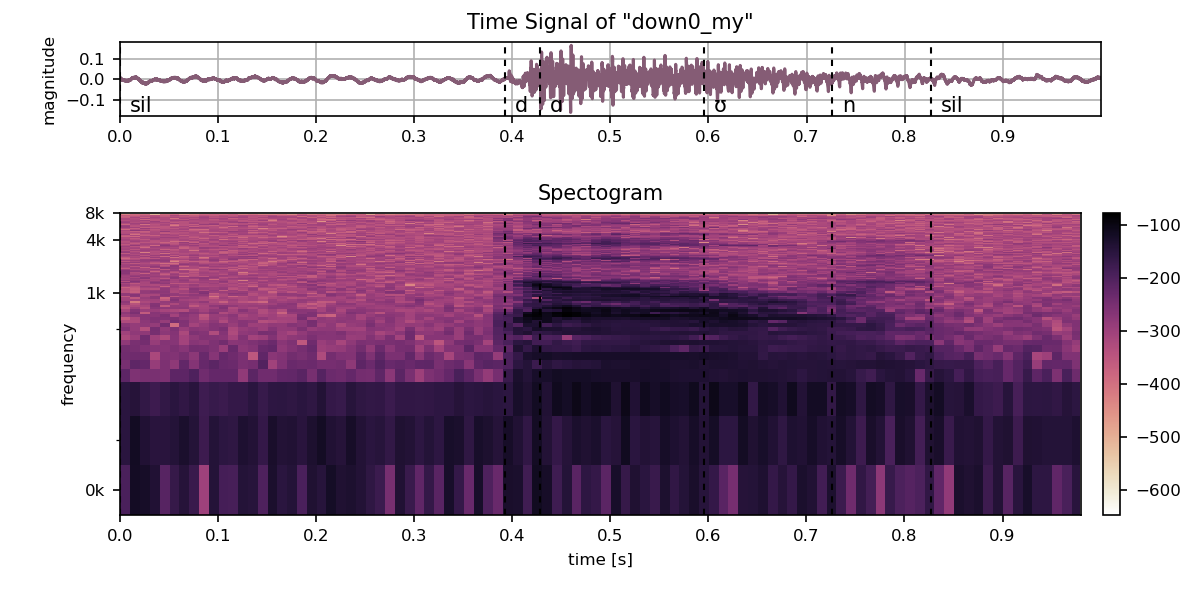
\includegraphics[width=0.45\textwidth]{./3_signal/figs/signal_spec-log_down0_my}}
    \subfigure[go]{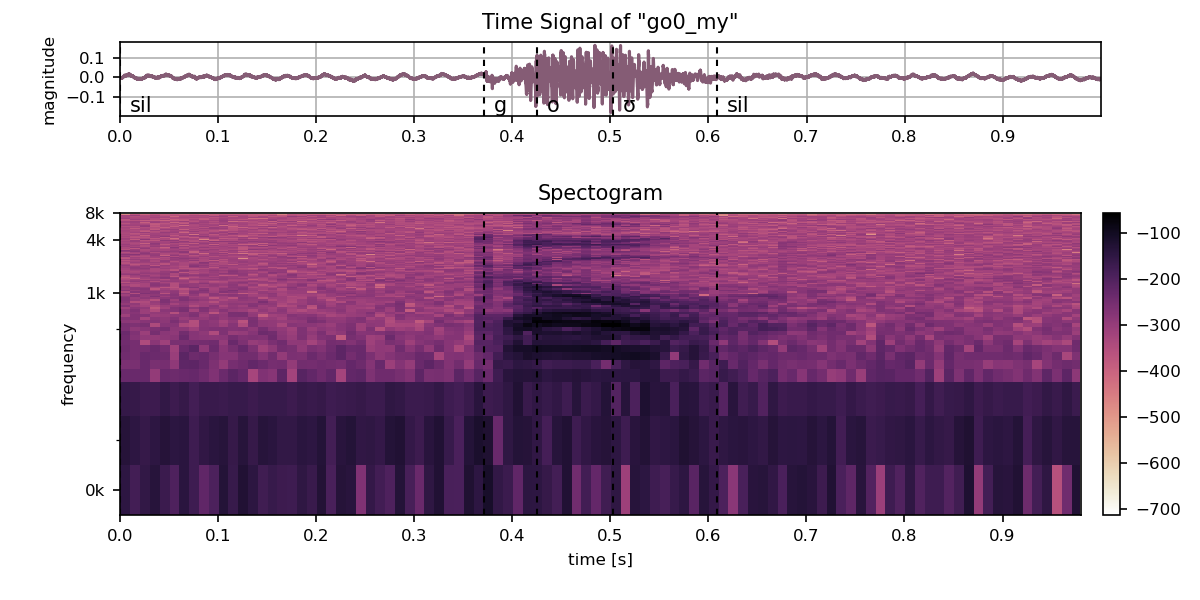
\includegraphics[width=0.45\textwidth]{./3_signal/figs/signal_spec-log_go0_my}}
  \caption{Spectrogram logarithmic scaled.}
  \label{fig:signal_spec_log_examples}
\end{figure}
\FloatBarrier
\noindent

Now it is possible to see some interesting structures and movements in the spectrograms in the frequency axis over time.
Still it is possible to improve the visualization of the spoken command words with a better compression scheme, such as the Mel Frequency Cepstral Coefficients, explained in the next section.